\chapter*{Apendiks A :\\ Kalkulus Diferensial dan Kalkulus Integral}
\section{Kalkulus Diferensial}
Fenomena fisis seringkali berurusan dengan sesuatu yang berubah terhadap waktu atau dengan kata lain berubah secara kontinu. Matematika kalkulus digunakan untuk berurusan dengan hal-hal yang berkenaan dengan perubahan kontinu. Kalkulus berhubungan dengan limit. Untuk memahami ide tentang limit, bayangakan kita memiliki urutan bilangan $l_1, l_2, l_3,...$ yang nilainya semakin dekat dan semakin dekat dengan sebuah nilai $L$. Sebagai contoh: 0.9, 0.99, 0.999, 0.9999,..... Dapat dikatakan bahwa limit dari urutan ini adalah sama dengan 1. Tidak ada satu pun dari angka-angka tersebut yang sama dengan 1, akan tetapi semakin lama semakin mendekati nilai 1. Jika ide ini digunakan pada fungsi yang berubah sejalan dengan waktu $f(t)$, maka $L$ adalah limit dari fungsi ketika $t$ mendekati nilai tertentu, misalnya $a$.
%--------------------------------------------------------------
\begin{equation}
\lim_{t\rightarrow a}f(t)=L 
\end{equation}
%--------------------------------------------------------------
Kalkulus diferensial berhubungan dengan laju perubahan fungsi $\Delta f$ terhadap perubahan waktu $\Delta t$. Laju perubahan didefinisikan sebagai rasio dari perubahan fungsi $\Delta f$ terhadap perubahan waktu $\Delta t$. Sepanjang interval $\Delta t$, fungsi berubah dari $f(t)$ menjadi $f(t+\Delta t)$, sehingga
\begin{equation}
\Delta f = f(t+\Delta t) - f(t)
\end{equation}
%--------------------------------------------------------------
\begin{figure}[!h]
\centering
\includegraphics[scale=0.6]{pict/differentialgraph.pdf}
\caption{Grafik fungsi yang berubah terhadap waktu, $\Delta f$ menunjukkan perubahan dalam fungsi sedangkan $\Delta t$ menunjukkan perubahan dalam waktu}\label{differential}
\end{figure}
%--------------------------------------------------------------
Untuk mendefinisikan laju perubahan pada satu waktu $t$ secara lebih akurat, kita harus menyusutkan $\Delta t$ pada Gambar 1.1 sampai nol. Tentu saja jika kita menyusutkan $\Delta t$ hingga nol maka $\Delta f$ juga akan menjadi nol. Akan tetapi, jika kita membagi $\Delta f$ dengan $\Delta t$ maka rasio/pembagian tersebut akancenderung menuju sebuah limit. Limit tersebut adalah turunan/derivatif dari fungsi $f(t)$ terhadap waktu $t$.
\begin{equation}
\label{sec:turunan}
\frac{df}{dt}=\lim_{\Delta t \rightarrow 0} \frac{\Delta f}{\Delta t}=\lim_{\Delta t \rightarrow 0} \frac{f(t + \Delta t)-f(t)}{\Delta t}.
\end{equation}
Sebagai contoh kita hitung turunan dari fungsi $f(t)=t^2$. Kita gunakan persamaan~\ref{sec:turunan} untuk menghitungnya, dimulai dari :
\[
f(t+\Delta t)=(t+\Delta t)^2=t^2+2t\Delta t + \Delta t^2
\]
kemudian kurangkan dengan $f(t)$
\begin{align*}
f(t+\Delta t)-f(t)&=t^2+2t\Delta t + \Delta t^2 - t^2\\
&=2t\Delta t + \Delta t^2.
\end{align*}
Dengan membaginya dengan $\Delta t$, kita dapatkan:
\begin{align*}
\frac{f(t + \Delta t)-f(t)}{\Delta t}&=\frac{2t\Delta t + \Delta t^2}{\Delta t}\\
&=2t+\Delta t.
\end{align*}
Pembagian ini akan menghasilkan limit jika $\Delta t \rightarrow 0$:
\begin{align*}
\lim_{\Delta t\rightarrow 0}\frac{f(t+\Delta t)-f(t)}{\Delta t}&=\lim_{\Delta t \rightarrow 0} 2t + \Delta t\\
&= 2t.
\end{align*} 
Jadi, turunan dari $t^2$ adalah
\[
\frac{d(t^2)}{dt}=2t
\]
Selanjutnya untuk fungsi dengan perpangkatan secara umum $f(t)=t^n$, turunannya dapat dihitung dengan memanfaatkan teorema binomial
\[
(a+b)^n=a^n+na^{n-1}b+\frac{n(n-1)}{2}a_{n-2}b^2+\frac{n(n-1)(n-2)}{3}a^{n-3}b^3+...+b^n.
\] 
Dengan menggunakan teorema binomial ini kita dapat menghitung $f(t+\Delta t)$,
\begin{align*}
f(t+\Delta t)&=(t+\Delta t)^n\\
&=t^n+nt^{n-1}\Delta t+...
\end{align*}
pengurangan dengan $f(t)$ menghasilkan
\begin{align*}
\Delta f&= f(t+\Delta t)-f(t)\\
&= t^n+nt^{n-1}\Delta t+\frac{n(n-1)}{2}t{n-2}\Delta t^2+...-t^n\\
&=nt^{n-1}\Delta t+\frac{n(n-1)}{2}t^{n-2}\Delta t^2+...
\end{align*}
Kemudian membaginya dengan $\Delta t$,
\[
\frac{\Delta f}{\Delta t}=nt^{n-1}+\frac{n(n-1)}{2}t^{n-2}\Delta t+...
\]
Dengan $\Delta t \rightarrow 0$ maka semua bagian yang mengandung $\Delta t$ akan menyusut menjadi nol dan menghasilkan sebuah limit
\begin{equation}
\frac{d(t^n)}{dt}=nt^{n-1},
\end{equation}
yang merupakan rumusan umum praktis untuk menyelesaikan turunan fungsi perpangkatan. $n$ di sini tidak terbatas pada bilangan bulat, tetapi juga untuk bilangan real apapun atau bahkan bilangan kompleks.

Beberapa aturan dalam turunan:
\begin{enumerate}
\item Turunan dari sebuah konstanta (konstanta adalah angka apapun, baik bilangan bulat maupun bilangan real) adalah sama dengan nol. Hal ini benar menurut pengertian turunan, yaitu bahwa turunan adalah laju perubahan, dan sebuah konstanta tidak akan berubah:
\[
\frac{dc}{dt}=0
\]
\item Turunan dari sebuah konstanta dikalikan dengan sebuah fungsi adalah konstanta tersebut dikalukan turunan dari fungsi:
\[
\frac{(cf)}{dt}=c\frac{df}{dt}
\]
\item Penjumlahan dari dua fungsi $f(t)$ dan $g(t)$ adalah juga berupa fungsi dan turunannya diberikan oleh:
\[
\frac{d(f+g)}{dt}=\frac{d(f)}{dt}+\frac{d(g)}{dt}.
\]
Aturan ini disebut dengan \textit{aturan penambahan} atau \textit{sum rule}.
\item Hasil kali dari dua fungsi adalah juga berupa fungsi dan turunannya adalah:
\[
\frac{d(fg)}{dt}=f(t)\frac{d(g)}{dt}+g(t)\frac{d(f)}{dt}.
\]
Aturan ini disebut \textit{aturan hasil kali}.
\item Jika kita memiliki dua fungsi, dimana $g(t)$ adalah sebuah fungsi dari $t$ dan $f(g)$ adalah fungsi dari $g$, yang membuat $f$ secara tidak langsung merupakan fungsi dari $t$. Maka untuk menurunkan fungsi semacam ini pertama kita harus turunkan terlebih dahulu fungsi $g(t)$ untuk kemudian barulah menurunkan $f(g)$:
\[
\frac{df}{dt}=\frac{df}{dg}\frac{dg}{dt}
\]
Aturan ini disebut dengan \textit{aturan rantai}. Hal yang penting dalam aturan rantai adalah bahwa kita harus menemukan fungsi perantara $g(t)$ untuk dapat menyederhanakan $f(t)$ dan membuatnya menjadi $f(g)$. Sebagai contoh, kita ambil fungsi $f(t)=\ln t^3$. Dalam fungsi ini $t^3$ bisa menjadi sebuah masalah. Kita ambil $t^3$ di dalam logaritma sebagai fungsi perantara, $g=t^3$. Sehingga sekarang kita memiliki $f(g)=\ln g$. Turunan kedua fungsi adalah:
\begin{align*}
\frac{df}{dt}&=\frac{1}{g}, dan\\
\frac{dg}{dt}&=3t^2.
\end{align*}
Dengan menggunakan aturan rantai, kita dapatkan:
\begin{align*}
\frac{df}{dt}&=\frac{df}{dg}\frac{dg}{dt}\\
&=\frac{3t^2}{g}.
\end{align*}
Substitusi $g=t^3$ menghasilkan turunan dari fungsi $f(t)$ terhadap waktu $t$
\[
\frac{df}{dt}=\frac{3t^2}{t^3}=\frac{3}{t}
\]   
\end{enumerate}
\section{Kalkulus Integral}
Jika kalkulus diferensial berhubungan dengan laju perubahan. kalkulus integral berhubungan dengan jumlahan dari banyak bagian-bagian kecil. Masalah utama dalam kalkulus integral adalah menghitung luasan dibawah kurva yang didefinisikan oleh sebuah fungsi $f(t)$. Misalkan kita ingin menghitung luasan dibawah kurva fungsi $f(t)$ dengan batasan dari a sampai b. Maka sebagai pendekatan kita dapat pecah-pecah luasan tersebut ke dalam bagian-bagian yang lebih kecil berbentuk persegi panjang dengan masing-masing memiliki ukuran yang sama, seperti terlihat pada gambar 1.2.
%-------------------------------------------------------------- 
\begin{figure}[!h]
\centering
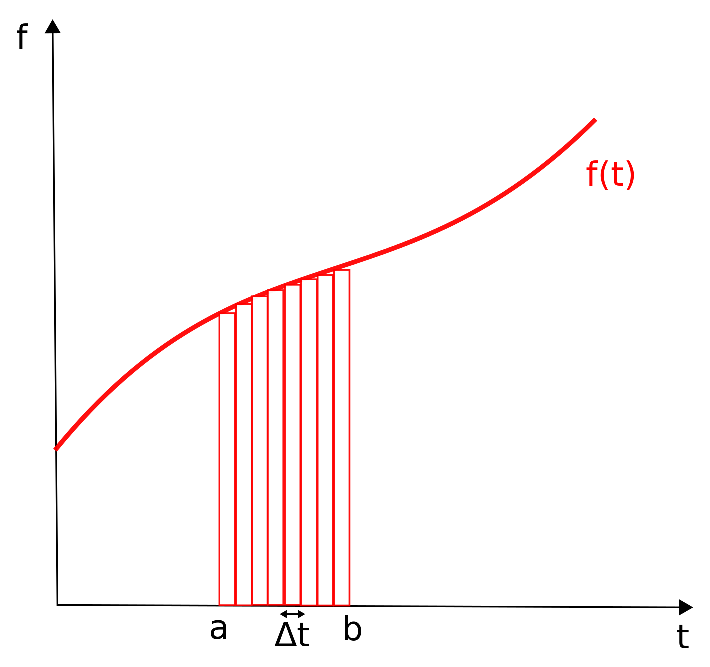
\includegraphics[scale=0.6]{pict/integralgraph.eps}
\caption{Grafik fungsi yang berubah terhadap waktu, Luasan di bawah kurva fungsi $f(t)$ dibagi-bagi kedalam banyak sub-luasan lebih kecil berbentuk persegi panjang}\label{integral}
\end{figure}
%--------------------------------------------------------------
Lebar dari persegi panjang ini adalah $\Delta t$ dan tingginya merupakan nilai lokal dari fungsi $f(t)$. Luasan dari sebuah persegi panjang tersebut adalah:
\[
\delta A=f(t)\Delta t
\]
Sekarang kita jumlahkan tiap-tiap persegi panjang ini sehingga mendekati luasan di bawah kurva dari a ke b.
\[
A=\sum^N_i f(t_i)\Delta t,
\]
$N$ di sini adalah banyaknya bagian-bagian persegi panjang. Untuk memperoleh hasil yang tepat dari luasan di bawah kurva ini, maka kita susutkan $\Delta t$ hingga menjadi nol dan jumlah dari persegi panjang menjadi tak berhingga. Integral tertentu antara $t=a$ dan $t=b$ dituliskan sebagai
\[
A=\int^b_a f(t) dt =\lim_{\Delta t \rightarrow 0} \sum_i f(t_i) \Delta t.
\]
Tanda integral $\int$, disebut \textit{summa}, menggantikan tanda penjumlahan sigma, dan $\Delta t$ digantikan oleh $dt$. Fungsi $f(t)$ disebut sebagai \textit{integrand}.

Jika kita ganti batasan $b$ dengan nilai variabel $T$ sehingga integrasi menjadi tak tentu. 
\[
\int^T_a f(t) dt
\]
Integral ini direpresentasikan dalam fungsi $F(T)$. Fungsi $F(T)$ mendefinisikan integral tak tentu dari fungsi $f(t)$, biasa ditulis dengan
\begin{equation}
F(T)=\int f(t) dt.
\end{equation}

Hubungan antara integral dan turunan bersifat resiprokal, yang berarti bahwa turunan dari integral adalah \textit{integrand} itu sendiri
\[
\frac{dF}{dt}=f(t).
\]
Hal ini dapat dibuktikan dengan menambahkan perubahan bagian kecil persegi panjang pada $T$ dari $T$ sampai $T+\Delta t$, sehinggga kita memiliki integral baru
\[
F(T+\Delta t)=\int^{T+\Delta t}_a f(t)dt.
\]  
Dengan penambahan sebuah persegi panjang Perbedaan $F(T+\Delta t)-F(T)$ tak lain hanyalah luasan dari persegi panjang tambahan itu sendiri
\[
F(T+\Delta t)-F(T)=f(T)\Delta t
\]
Pembagian dengan $\Delta t$ menghasilkan
\[
\frac{F(T+\Delta t)-F(T)}{\Delta t}=f(T).
\]
Jika kita ambil limit dimana $\Delta t \rightarrow 0$, maka
\[
\frac{dF}{dT}=\lim_{\Delta t \rightarrow 0} \frac{F(T+\Delta t)-F(T)}{\Delta t}=f(T).
\]  
Kita dapat menyederhanakan ini dengan mengabaikan perbedaan antara $t$ dan $T$,
\[
\frac{dF}{dt}=f(t).
\]

Untuk lebih memahaminya kita coba menemukan integral dari fungsi perpangkatan $f(t)=t^n$
\[
F(t)=\int f(t)dt=\int t^n dt.
\]
Dari hubungan antara $F$ dan $f$
\[
f(t)=\frac{dF(t)}{dt}
\]
atau
\[
t^n=\frac{dF(t)}{dt}.
\]
Hal yang harus kita lakukan adalah menemukan fungsi $F$ yang turunannya adalah $t^n$.\\
Dari sub-bab sebelumnya tentang kalkulus diferensial, kita menemukan bahwa untuk apapun nilai $m$,
\[
\frac{d(t^m)}{dt}=mt^{m-1}
\].
Jika kita substitusikan $m=n+1$, maka akan menjadi
\[
\frac{d(t^{n+1})}{dt}=(n+1)t^n
\]
atau, dengan membagi dengan $n+1$,
\[
\frac{d(\frac{t^{n+1}}{n+1})}{dt}=t^n.
\]
Sehingga kita menemukan bahwa $t^n$ adalah turunan dari $\frac{t^{n+1}}{n+1}$. Dapat dituliskan sebagai
\[
F(t)=\int t^n dt=\frac{t^{n+1}}{n+1}.
\]

Secara umum teorema dasar dari kalkulus dapat dituliskan sebagai
\begin{equation}
\int^b_af(t)dt=F(t)\vert^b_a=F(b)-F(a).
\end{equation}

Beberapa rumus integrasi antara lain:
\begin{itemize}
\item $\int cdt=ct$
\item $\int cf(t)dt=c\int f(t) dt$
\item $\int t dt=\frac{t^2}{2}+c$
\item $\int t^2dt=\frac{t^3}{3}+ c$
\item $\int t^ndt=\frac{t^{n+1}}{n+1}+c$
\item $\int \sin tdt=-\cos t+c$
\item $\int \cos tdt=\sin t+c$
\item $\int e^t dt=e^t$
\item $\int \frac{dt}{t}=\ln t+c$
\item $\int [f(t)\pm g(t)]dt=\int f(t) dt \pm \int g(t) dt$. 
\end{itemize}

\subsubsection{Integrasi parsial}
Integrasi parsial adalah salah satu \textit{tool} untuk menyelesaiakn perhitungan integral yang rumit. Integral parsial merupakan balikan dari \textit{aturan hasil kali} dari turunan. Kembali kita tinjau \textit{aturan hasil kali}
\[
\frac{d[f(x)g(x)]}{dx}=f(x)\frac{dg(x)}{dx}+g(x)\frac{df(x)}{dx}.
\]
Mengintegralkan kedua sisi dari presamaan dari $a$ sampai $b$ menghasilkan
\begin{align}
\int_a^b\frac{d[f(x)g(x)]}{dx}&=\int_a^bf(x)\frac{dg(x)}{dx}+\int_a^b g(x) \frac{f(x)}{dx}\\
f(x)g(x)\vert_a^b - \int_a^b f(x) \frac{dg(x)}{dx} &= \int_a^b g(x) \frac{df(x)}{dx}.
\end{align}
Jika $f(x)$ direpresentasikan dengan $u$ dan $g(x)$ dengan $v$, sehingga $df(x)/dx=du$ dan $dg(x)/dx=dv$, maka substitusi pada persamaan (1.8) menghasilkan
\begin{equation}
uv-\int udv = \int vdu,
\end{equation} 
yang merupakan rumusan praktis dari integrasi parsial. Sebagai contoh, kita hitung integral dari $x\cos x$ dari 0 sampai $\pi/2$
\[
\int_0^{\pi/2} x \cos x dx,
\]
dengan menggunakan persamaan (1.9) ambil $x$ sebagai $v$ dan $\cos x dx$ sebagai $du$
\begin{align*}
v&=x,  dv=dx\\
du&=\cos x dx,   u=\sin x.
\end{align*}  
Substitusi ke persamaan (1.9) menghasilkan
\begin{align*}
\int_0^{\pi /2} x \cos x dx&=x \sin x\vert_0^{\pi /2}-\int_0^{\pi /2} \sin x dx\\
&= \frac{\pi}{2} \sin \frac{\pi}{2}+\cos \frac{\pi}{2}\\
&=\frac{\pi}{2}.
\end{align*}
